\documentclass{article} % For LaTeX2e
\usepackage{cos424,times}
\usepackage{url}
\usepackage{graphicx}
\usepackage{hyperref}
\usepackage{amsmath, bbold}
\usepackage{bm}

\newcommand{\e}{\text{e}}
\newcommand{\bt}{\mathbf}

\title{Kaggle Competition: Flavors of Physics}


\author{
Kenan Farmer\\
Computer Science\\
\texttt{kfarmer@} \\
\And
Charles Stahl \\
Physics \\
\texttt{cnstahl@} \\
\And
Meir Hirsch\\
Computer Science \\
\texttt{ehirsch@} \\
}

\newcommand{\fix}{\marginpar{FIX}}
\newcommand{\new}{\marginpar{NEW}}

\begin{document}

\maketitle

\subsection*{Introduction}
This will be a classification problem using all real data.
\subsection*{Data Description}
\subsection*{Methodologies to Explore}
\subsection*{Metrics}
We will follow the guide line of the competition admins for measuring our analysis performance. The main metric we will use to evaluate our methodologies is the Weighted Area under the ROC curve. The ROC curve is divided into sections based on the True Positive Rate (TPR). To calculate the total area, multiply the area with TPR in [0., 0.2] by weight 2.0, the area with TPR in [0.2, 0.4] by 1.5, the area with TPR [0.4, 0.6] with weight 1.0, and the area with TPR [0.6, 0.8] with weight 0.5. Anything above a TPR of 0.8 has weight 0. This metric is illustrated in the following figure:
\begin{center}
	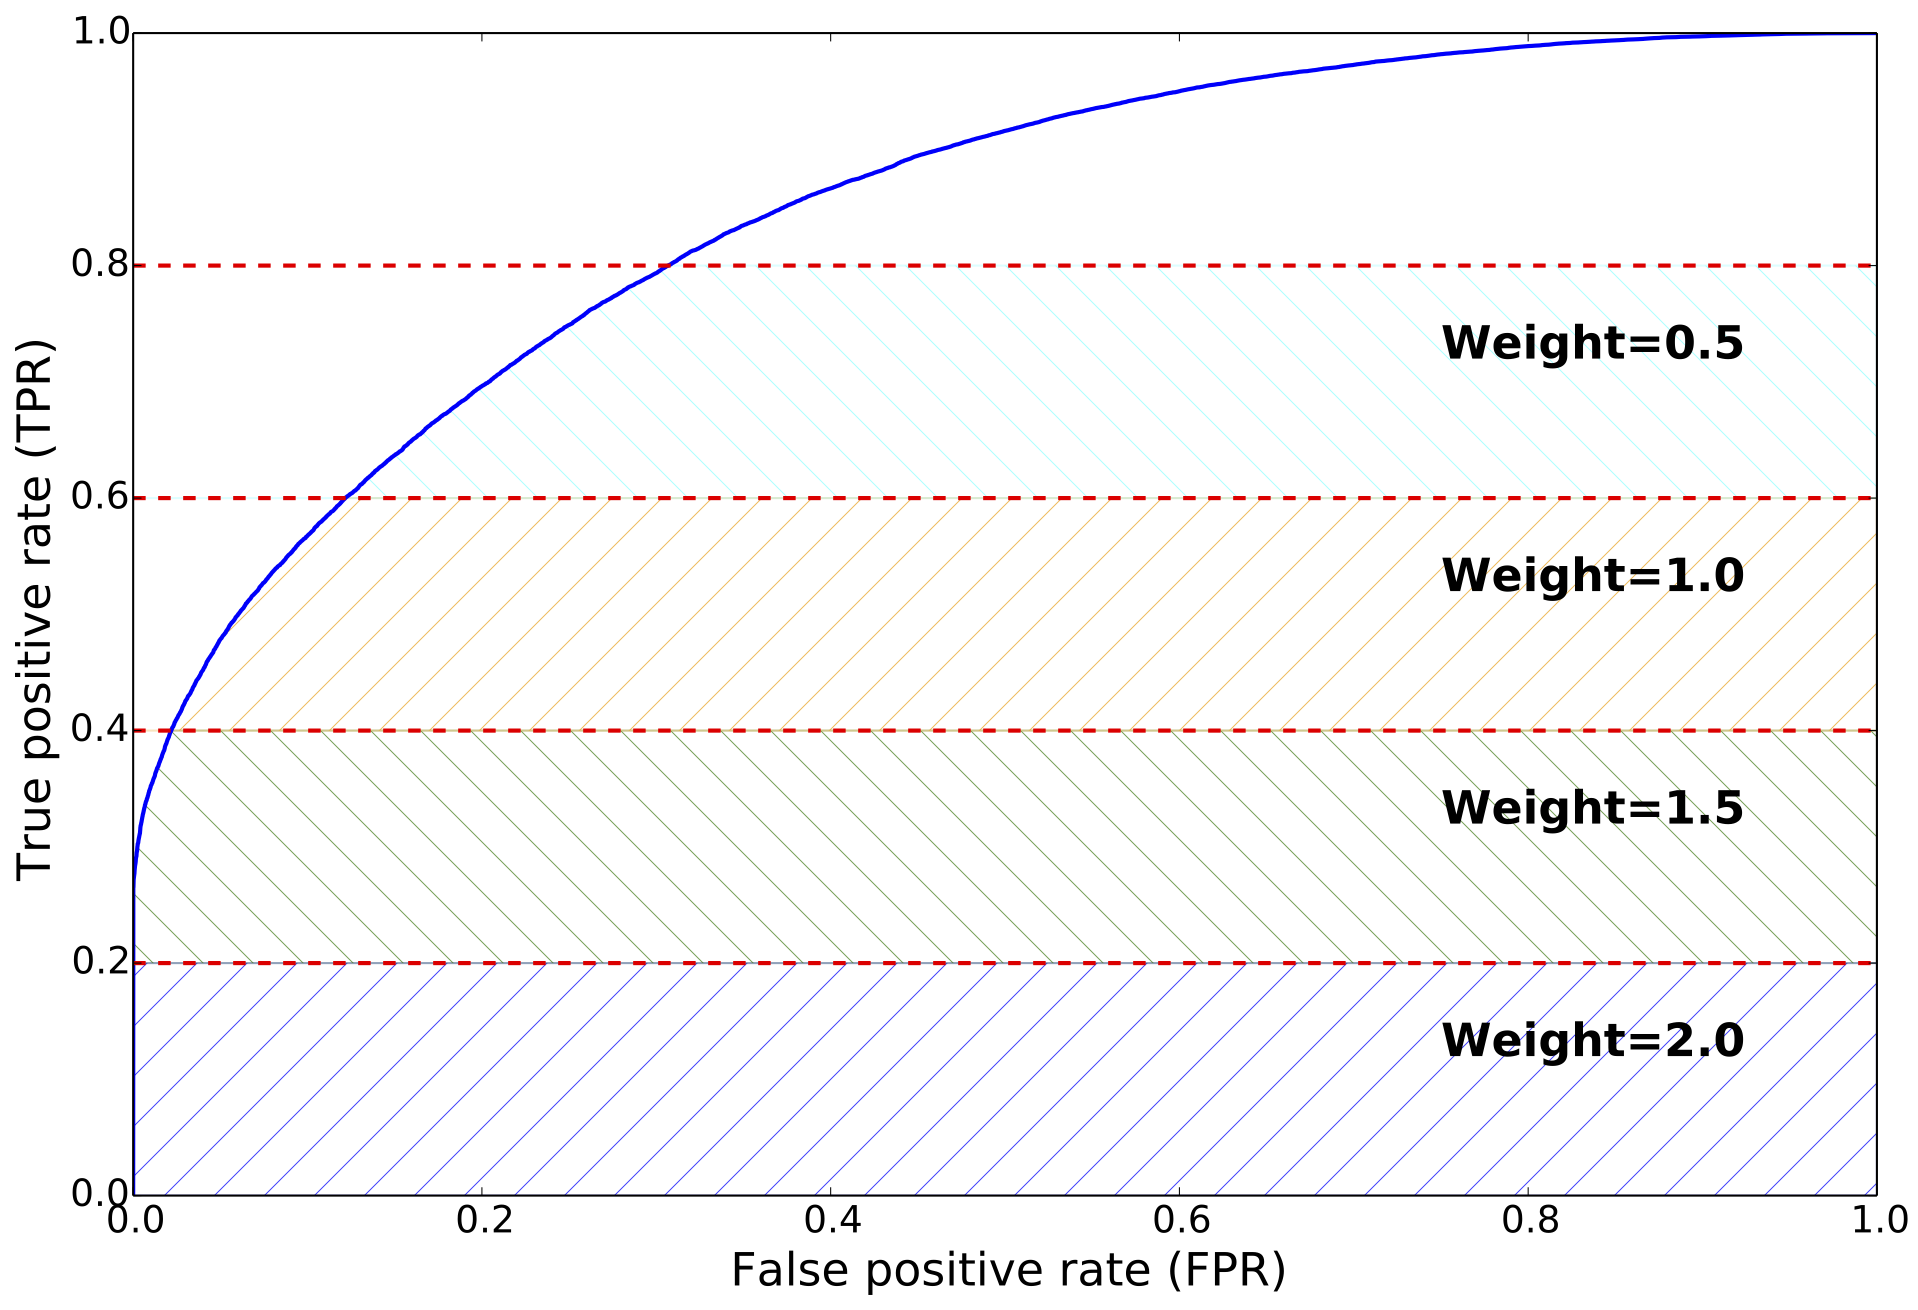
\includegraphics[scale = .3]{roc_optimistic}
\end{center} 
These weights were chosen to match the evaluation methodology used by CERN scientists.\cite{kaggleComp}.

\end{document}
